\section{Einleitung}
In Bezug auf den Schweregrad gab es in der Schweiz seit der Spanischen Grippe im Jahr 1918 keine vergleichbaren Pandemien mehr. Kasbar Staub bezeichnet den Zeitraum von 1918 - 2020, in welchem es keine verheerenden Pandemien für die Schweiz gab, als \textit{Pandemic Gap in Switzerland} (siehe Abbildung \ref{fig:pandemic_gap_switzerland}). Mit dem Auftreten der neusten Pandemie im Jahr 2019, bekannt unter dem Namen \gls{covid19} steht die Schweiz, sowie auch der Rest der Welt vor neuen Herausforderungen.

\begin{figure}[h]
    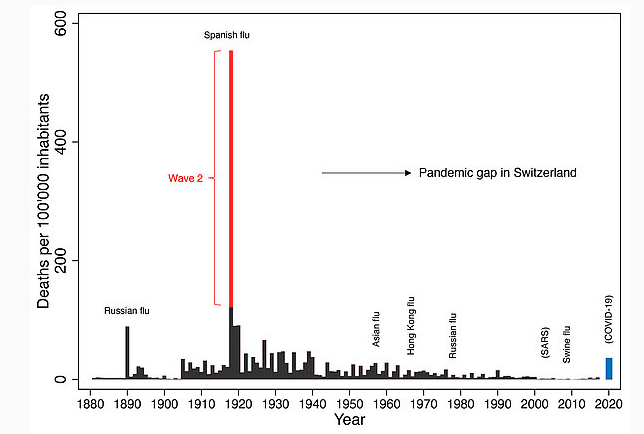
\includegraphics[width=12cm]{images/pandemic_gap_switzerland.png}
    \centering
    \caption{Visualisierung Pandemic Gap in Switzerland ~\citep{switzerland_pandemic_gap}}
    \label{fig:pandemic_gap_switzerland}
\end{figure}


Gemäss der Studie von Statista, welche Epidemien und Pandemien aus dem Jahr 1918 bis 2021 miteinander vergleicht, hebt sich Corona mit rund 5000 krankheitsbedingten Todesfällen pro Tag merklich von anderen Virusvarianten ab (siehe Abbildung \ref{fig:daily_deaths_due_to_contamination}).

\begin{figure}[h]
    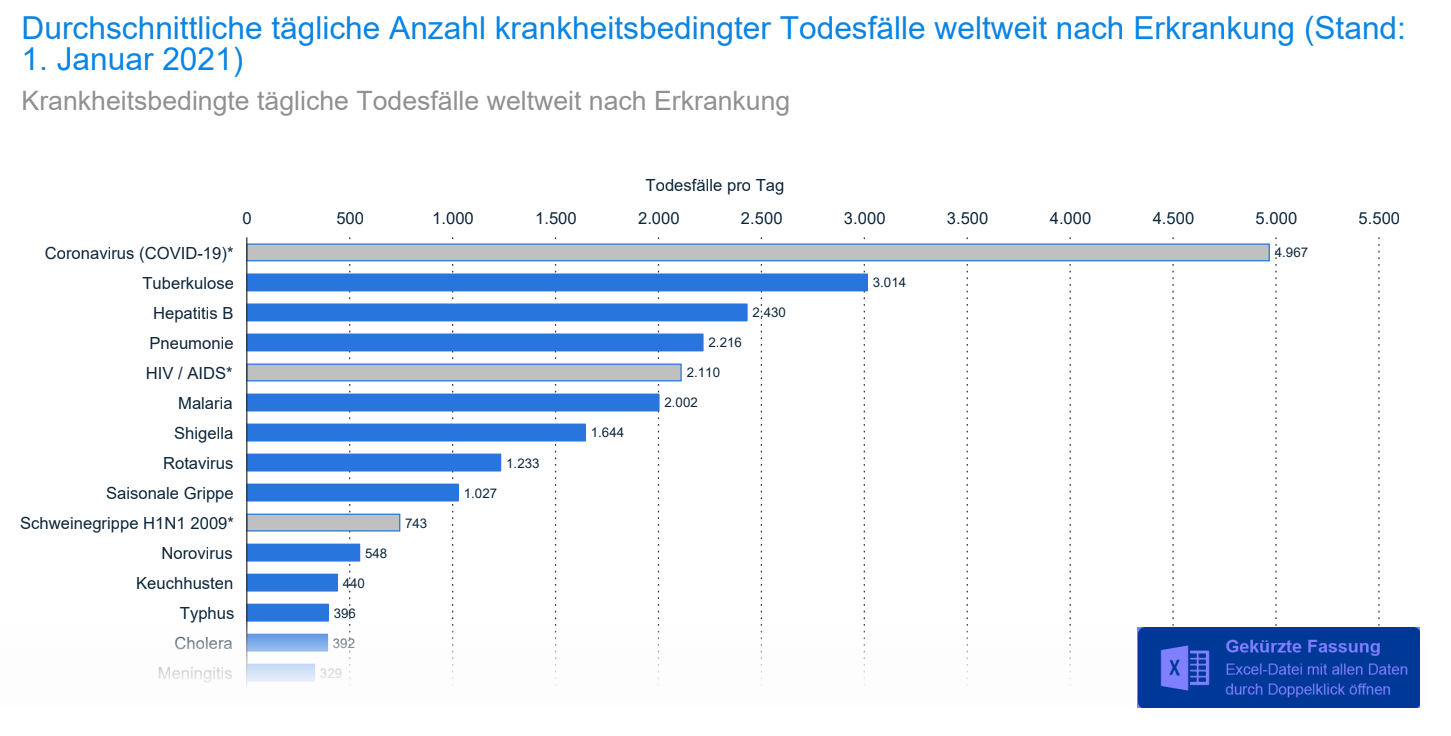
\includegraphics[width=12cm]{images/daily_deaths_after_contamination.png}
    \centering
    \caption{Durchschnittliche tägliche Anzahl krankheitsbedingter Todesfälle weltweit nach Erkrankung (Stand:
1. Januar 2021) ~\citep[S. 6]{worldwide_epidemic_cases_study}}
    \label{fig:daily_deaths_due_to_contamination}
\end{figure}

Ein zentrales Mittel zur Sensibilisierung der allgemeinen Bevölkerung in Bezug auf den Schweregrad der Pandemie sind hierbei \textbf{Datenvisualisierungen} und insbesondere \textbf{Dashboards}. Dies bestätigt ebenfalls Barbazza in seinem Paper, welche die Erfahrungen von 33 nationalen Teams in Bezug auf die Erstellung von Corona spezifische Dashboards im Rahmen einer qualitativen Studie auswertete. Gemäss dem Paper geht hevor, dass Regierungen in der europäischen WHO Region primär ein Dashboard nutzten, um Corona spezifische Daten der Öffentlichkeit mitzuteilen ~\citep[S. 2]{barbazza}. Barbazza identifizierte im Rahmen von qualitativ durchgeführten Experteninterviews mit Personen welche für die Erstellung von Dashboards verantwortlich waren zwei Problematiken. Zum einen wurden die Dashboards für die breite Öffentlichkeit und nicht für eine dedizierte Zielgruppe konzipiert, zum anderen gab es keine effiziente Möglichkeit um an das Feedback der Nutzergruppe zu gelangen ~\citep[S. 14-15]{barbazza}. Die vorliegende Arbeit untersucht diese Problematiken mit der Umsetzung eines Corona Dashboards für die Zielgruppe der Millenials.


\subsection{Stand der Forschung}
 Eine Studie von Statista zum Thema \gls{covid19} zeigt auf, dass die Suchbegriffe ``Corona`` sowie  ``\gls{covid19}`` sehr präsent sowohl bei Medienberichten als auch bei Google-Anfragen sind (siehe Abbildung \ref{fig:covid_term_public_media_presence}).
 
\begin{figure}[h]
    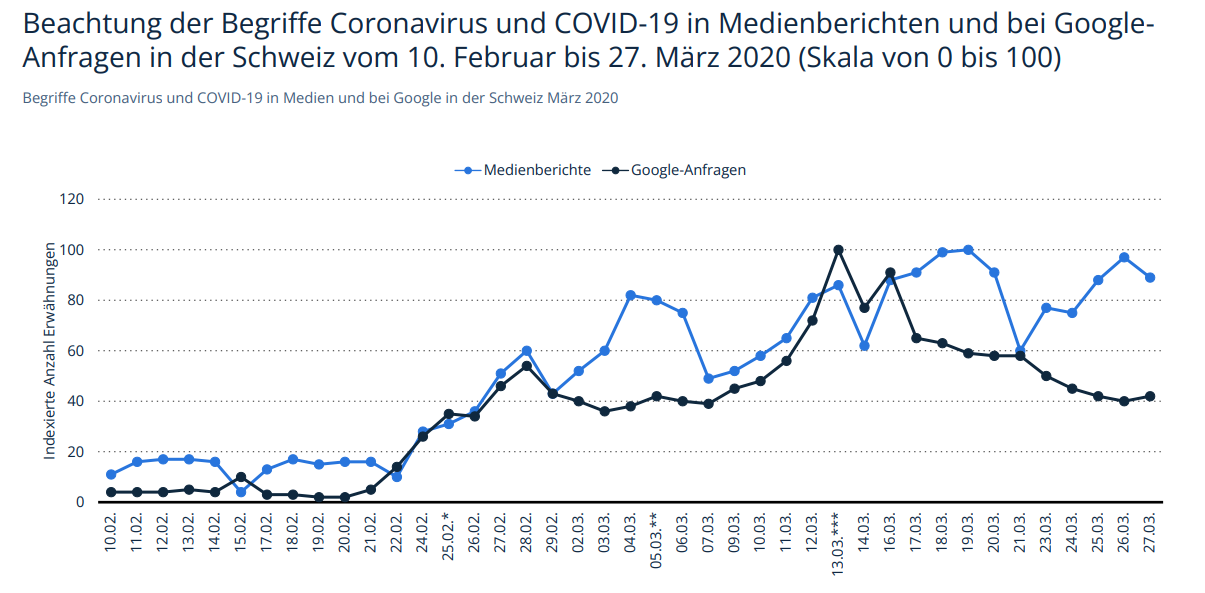
\includegraphics[width=12cm]{images/covid_term_public_media_presence.png}
    \centering
    \caption{Beachtung der Corona Begrifflichkeiten in Medienberichten und bei Google-Anfragen vom 10. Februar 2020 bis 27. März 2020 ~\citep[S. 50]{covid_term_public_media_presence}}
    \label{fig:covid_term_public_media_presence}
\end{figure}
 
Nachfolgend wird auf die wichtigsten bereits bestehenden Studien eingegangen, welche sich mit  \textbf{Datenvisualisierungen} sowie \textbf{Dashboards} im Zusammenhang mit Corona beschäftigen.
 
 \subsubsection{Die Landschaft der Corona Datenvisualisierungen} \label{ch:landscape_of_covid_data_visualization}
 Eine massgebende Studie um einen Überblick über die Landschaft der Corona Datenvisualisierungen zu erhalten, ist die Studie von Zhang. Bei dieser Studie wurden rund 668 Corona Datenvisualisierungen im Zeitraum vom 22. Januar bis zum 31. Juli 2020 analysiert. Ein wichtiges Auswahlkriterium bei diesen Visualisierungen war, dass die allgemeine Bevölkerung als Zielgruppe im Fokus stand. Anschliessend wurden diese Visualisierungen sowohl mittels \textit{deduktiver} als auch \textit{induktiver} Codierung in Form eines Codebooks zusammengefasst ~\citep[S. 3]{yixuan_zhang}. Nebst dem Codebook erstellte Zhang zudem ein Rahmenwerk zum Verständnis von Datenvisualisierungen in Krisenzeiten (siehe Abbildung \ref{fig:zhang_conceptual_framework}).
 
 
 \begin{figure}[h]
    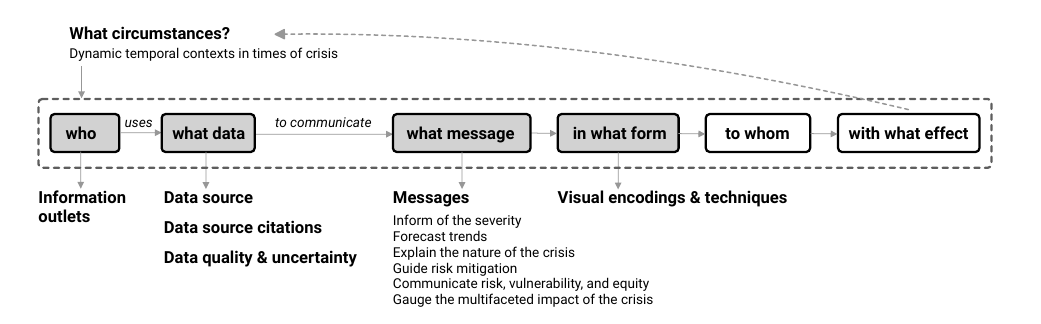
\includegraphics[width=12cm]{images/zhang_conceptual_framework.png}
    \centering
    \caption{Konzeptionelles Framework zum Verständnis von Datenvisualisierungen in Krisenzeiten ~\citep[S. 4]{yixuan_zhang}}
    \label{fig:zhang_conceptual_framework}
\end{figure}
 
 
 Die Studie von Zhang fokussierte sich hierbei primär auf die ersten vier Aspekte des Modells (who uses what data to communicate what message in what form). Im erstellten Codebook finden sich diese vier Aspekte ebenfalls wieder. Hierbei kann der Aspekt \textbf{who} mithilfe der Metainformationen ``Publisher`` sowie ``URL`` beantwortet werden (siehe Abbildung \ref{fig:zhang_codebook_metadata}).
 
 \begin{figure}[h]
    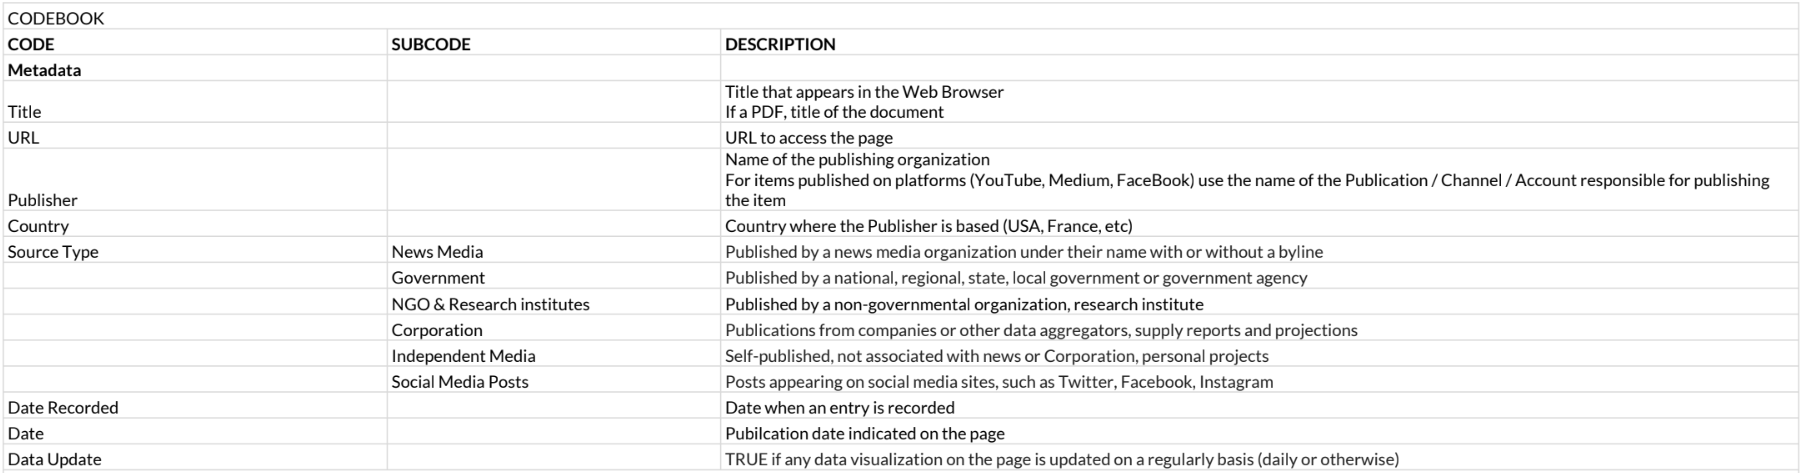
\includegraphics[width=12cm]{images/zhang_codebook_metadata.png}
    \centering
    \caption{Ausschnitt Metadaten aus dem Codebook von Zhang ~\citep{zhang_codebook}}
    \label{fig:zhang_codebook_metadata}
\end{figure}

Der Aspekt \textbf{what data} ist durch die Sektion ``Data Handling`` abgedeckt, welcher Informationen bezüglich der Datenquelle etc. aufweist (siehe Abbildung \ref{fig:zhang_codebook_data_handling}).

\begin{figure}[h]
    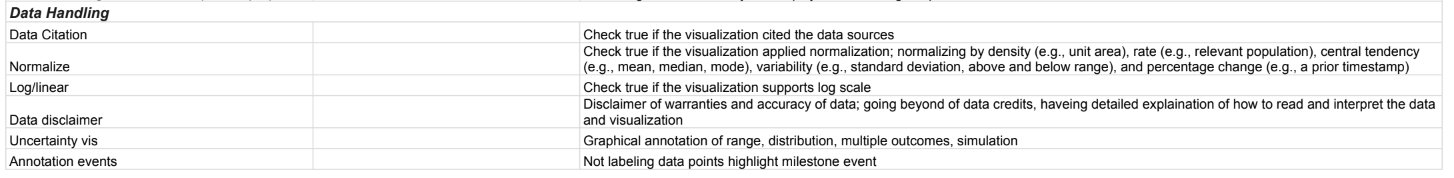
\includegraphics[width=12cm]{images/zhang_codebook_data_handling.png}
    \centering
    \caption{Ausschnitt Data Handling aus dem Codebook von Zhang ~\citep{zhang_codebook}}
    \label{fig:zhang_codebook_data_handling}
\end{figure}

 \textbf{What messages} sind durch die ``Intended Message`` Kategorie, welche mithilfe deduktiver sowie induktiver Codierung entstand, abgedeckt (siehe Abbildung \ref{fig:zhang_codebook_intended_message}).

\begin{figure}[h]
    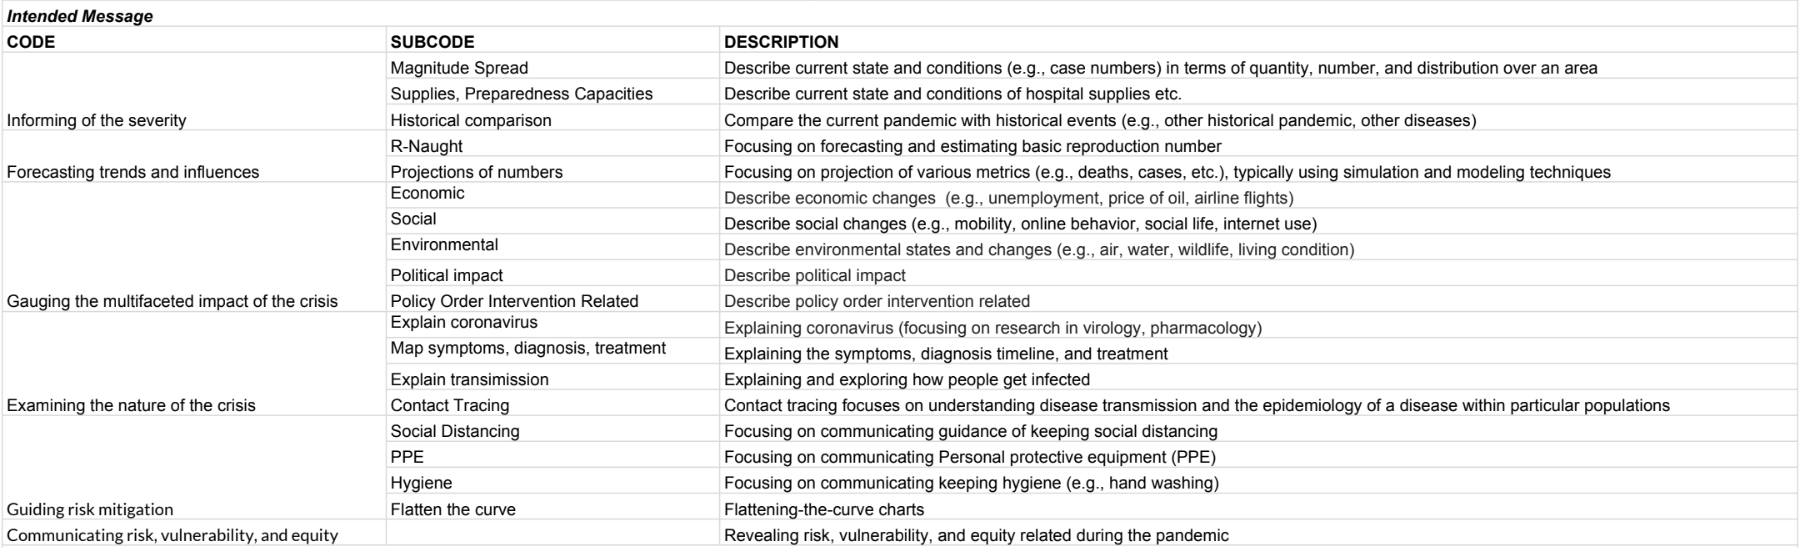
\includegraphics[width=12cm]{images/zhang_codebook_intended_message.png}
    \centering
    \caption{Ausschnitt Intended Message aus dem Codebook von Zhang ~\citep{zhang_codebook}}
    \label{fig:zhang_codebook_intended_message}
\end{figure}

 Der letzte Aspekt \textbf{in what form} kann ebenfalls aus dem Codebook entnommen werden. Zhang hat hierbei unter der Kategorie ``Type of Visualization`` verschiedene Visualisierungsarten wie zum Beispiel Liniendiagramme etc. aufgeführt (siehe Abbildung \ref{fig:zhang_codebook_type_of_visualization}).
 
 
\begin{figure}[h]
    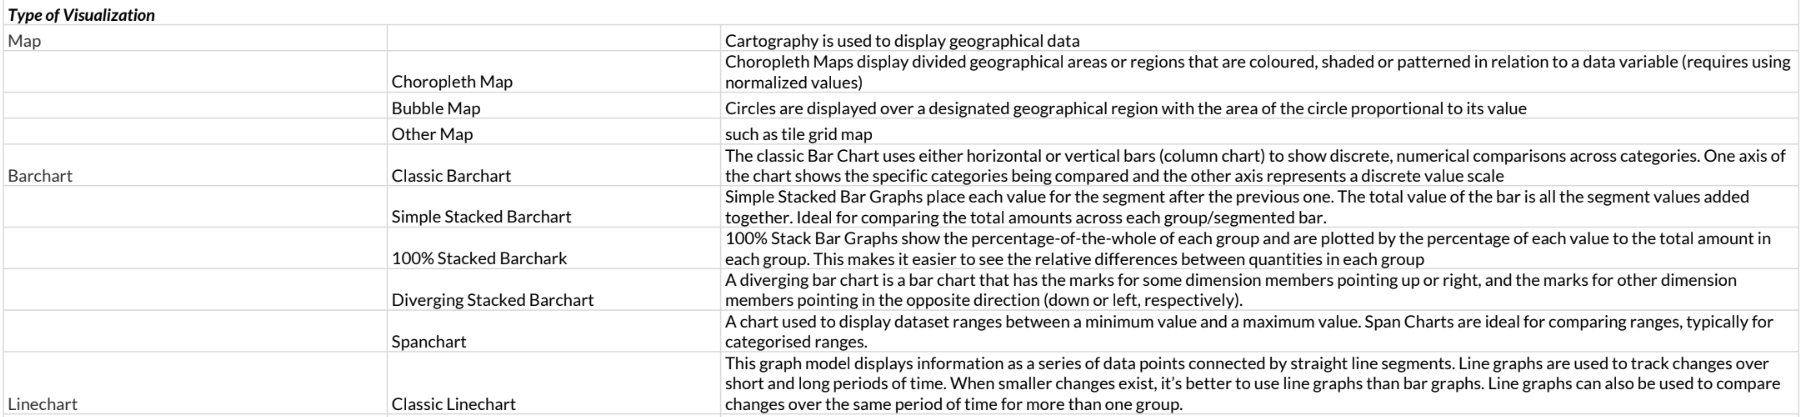
\includegraphics[width=12cm]{images/zhang_codebook_type_of_visualization.png}
    \centering
    \caption{Ausschnitt Type of Visualization aus dem Codebook von Zhang ~\citep{zhang_codebook}}
    \label{fig:zhang_codebook_type_of_visualization}
\end{figure}

Das Codebook bietet somit eine solide Grundlage um die Landschaft der Corona Datenvisualisierungen zu erfassen. Zudem kann es aufgrund seiner strukturierten Kategorien für weiterführende \textbf{Datenauswertungszwecke} verwendet werden.   
 
 
\subsubsection{Corona-Dashboards}
Barbazza führte in Bezug auf Corona Dashboards eine qualitative Studie durch, welche die Erfahrungen und Eindrücke von 33 nationalen Teams in Bezug auf die Konzeption und Umsetzung von Corona Dashboards untersuchte. Barbazza untersuchte hierbei zwei zentrale Hauptaspekte (siehe Abbildung \ref{fig:barbazza_method_design}). 


\begin{figure}[h]
    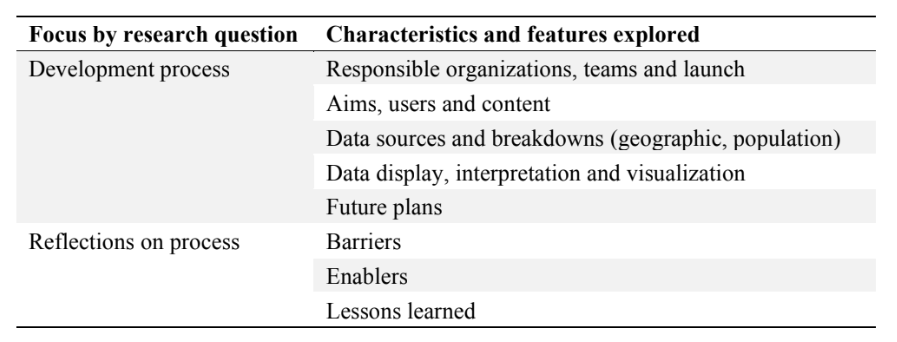
\includegraphics[width=12cm]{images/barbazza_method_design.png}
    \centering
    \caption{Hauptfokuspunkte der Studie von Barbazza ~\citep[S. 4]{barbazza}}
    \label{fig:barbazza_method_design}
\end{figure}

Zum einen wurde der Entwicklungsprozess eines Corona Dashboards analysiert. Nachfolgend wurden Barrieren (Dinge welche den Entwicklungsprozess behinderten), Enablers (Dinge welche den Entwicklungsprozess vorangetrieben haben) sowie Lessons learned identifiziert. Die Studie von Barbazza bietet somit eine gute Grundlage um das bestehende Feedback in Bezug auf Corona Dashboard Design einzuholen.

Anders als Barbazza fokussierte sich Ivankovi{\'c} hingegen explizit auf \textit{webbasierte} Dashboards. Konkret wurden hierbei Aspekte wie Funktion (Purpose), Inhalt und Daten (What) sowie die eigentliche Visualisierung (how they communicate COVID-19 data) untersucht. Aus den insgesamt 158 untersuchten Dashboards wurden anschliessend die Gemeinsamkeiten evaluiert. Hieraus entstanden 7 zentrale Merkmale von interaktiven webbasierten Dashboards (siehe Abbildung \ref{fig:ivankovic_characteristics_of_webbased_dashboards}). Diese Merkmale bildeten anschliessend die Grundlage, um die 158 untersuchten Dashboards zu bewerten ~\citep{ivankovic}. Ivankovi{\'c} bietet somit ein Bewertungsraster in Bezug auf interaktive, webbasierte Corona Dashboards an.


 \begin{figure}[h]
    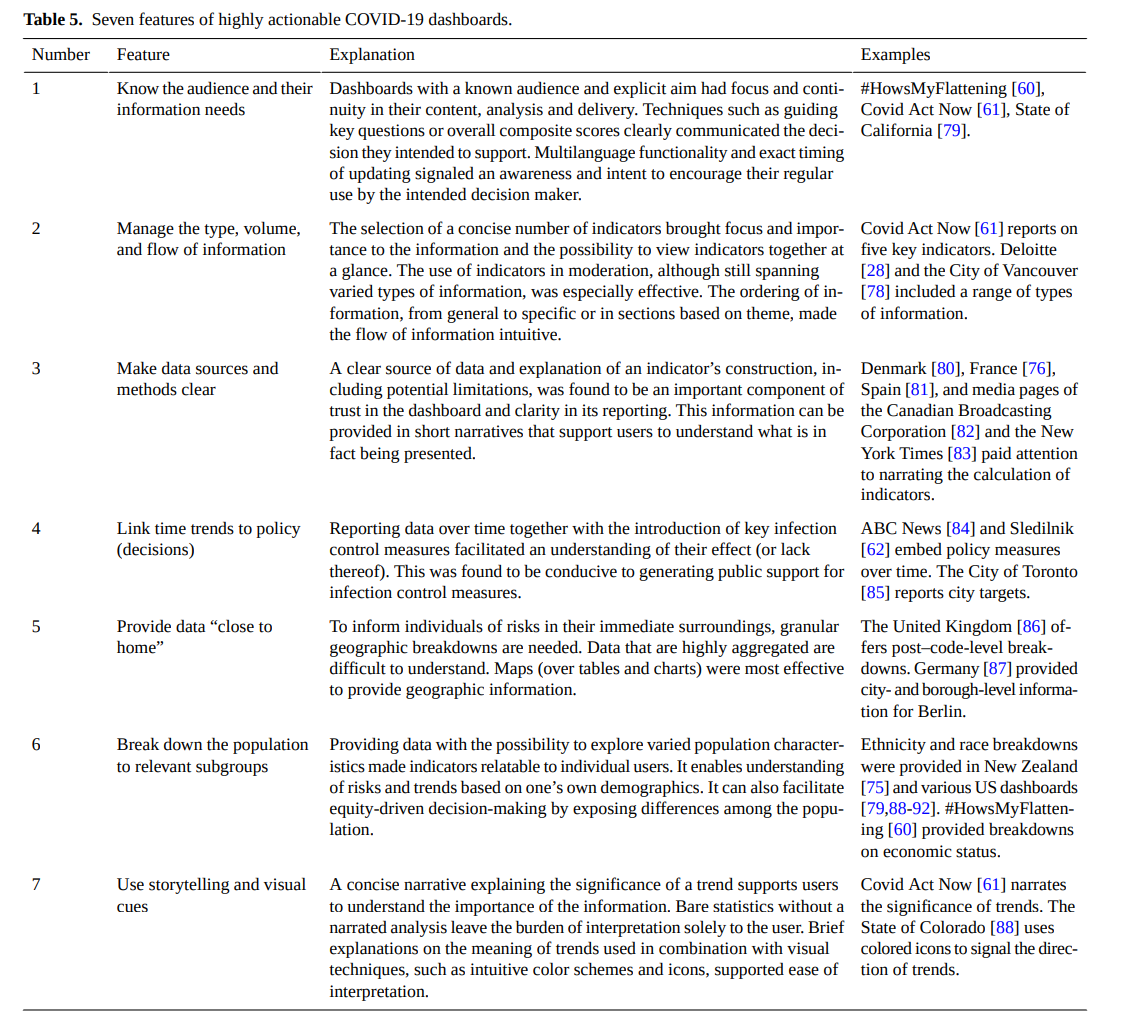
\includegraphics[width=10cm]{images/ivankovic_dashboard_characteristics.png}
    \centering
    \caption{Merkmale von interaktiven, webbasierten Dashboards gemäss Ivankovi{\'c} ~\citep[S. 12]{ivankovic}}
    \label{fig:ivankovic_characteristics_of_webbased_dashboards}
\end{figure}


\subsection{Themenabgrenzung und Zielsetzung}
Der Bereich der Datenvisualisierungen im Zusammenhang mit \gls{covid19} ist umfassend. Dashboards erlauben eine verdichtete Sicht auf die relevantesten Informationen, welche mit Hilfe von Datenvisualisierungen bereit gestellt werden können. Ein Problem welches Barbazza bereits in Ihrer Studie entdeckte, war dass die meisten Dashboards für eine allgemeine Zielgruppe ausgerichtet sind. Die vorliegende Arbeit hat daher zum Ziel, ein personalisierbares Dashboard für die Zielgruppe der Millenials zu entwickeln.

\subsection{Forschungsfrage}
Die vorliegende Arbeit möchte die Erstellung eines personalisierbaren Corona Dashboards für die Zielgruppe Millenials erforschen. Daher wurde folgende übergeordnete Fragestellung formuliert:

\begin{center}
\textbf{Wie stellen sich Millennials ein personalisierbares Corona Dashboard vor?}
\end{center}

Um diese Forschungsfrage abzudecken, wurden folgende untergeordnete Fragestellungen formuliert:

\begin{center}
\textbf{Welche Visualisierungsarten in Bezug auf Corona werden von Millennials gefordert?\\
(untergeordnete Forschungsfrage 1)}
\end{center}

\begin{center}
\textbf{Welche Informationen in Bezug auf Corona werden von Millennials gefordert?\\
(untergeordnete Forschungsfrage 2)}
\end{center}

\begin{center}
\textbf{Welche Personalisierungsmöglichkeiten werden von Millennials in Bezug auf Corona Dashboards gefordert?\\
(untergeordnete Forschungsfrage 3)}
\end{center}

\clearpage
\subsection{Methodische Vorgehensweise}
Da das Ziel der vorliegenden Arbeit die Erstellung eines personalisierbaren Corona Dashboards für Millenials ist, wurde als methodische Vorgehensweise das \gls{dsr} Modell nach Peffers gewählt, welches die Erstellung eines Artefakts zulässt (siehe Abbildung \ref{fig:peffers_dsr_model}).

\begin{figure}[h]
	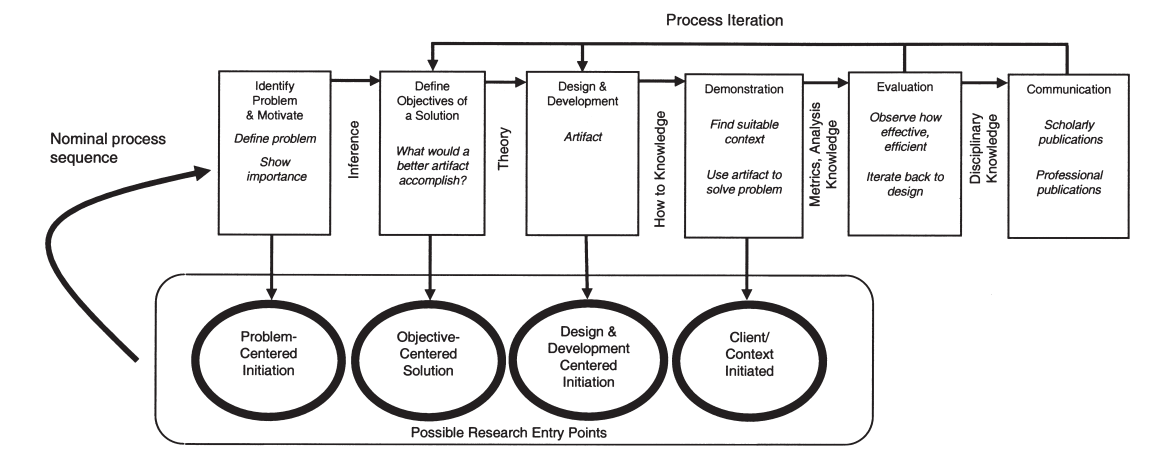
\includegraphics[width=14cm]{images/peffers_dsr_model.png}
	\centering
	\caption{DSR Modell nach Peffers ~\citep[S. 54]{peffers}}
	\label{fig:peffers_dsr_model}
\end{figure}

Das Modell bietet hierbei mehrere Einstiegsmöglichkeiten (siehe ``Possible Research Entry Points``). Der Einstiegspunkt für die vorliegende Arbeit bildet der Punkt \textbf{Design \& Development Centered Initiation}. Dies setzt zugleich auch den Zielfokus der Arbeit auf den Bereich Design und Entwicklung. Um diesen Kernbereich jedoch ausreichend erforschen zu können, werden im Verlaufe der Arbeit die ersten fünf Aktivitäten ``Identify Problem \& Motivation``, ``Define Objective \& Solution``, ``Design \& Development``, ``Demonstration`` sowie ``Evaluation`` behandelt.

\subsubsection{Problem Identification \& Motivation}
In der Aktivität ``Problem Identification \& Motivation`` wird das spezifische Problem, welches gelöst werden soll beschrieben sowie der Nutzen einer möglichen Lösung aufgezeigt ~\citep[S. 52]{peffers}. Als Grundlage für die Problemidentifiaktion dient hierbei die Studie von Barbazza, die Arbeit fokussiert sich hierbei auf die Barrieren in den Bereichen ``Nutzer`` sowie ``Software``. Hauptfokus ist die Erarbeitung eines Dashboards für die Zielgruppe Millenials.

\subsubsection{Define Objective \& Solution}
Bei dieser Aktivität geht es um die Definierung der Ziele ~\citep[S. 52]{peffers}. Hierbei werden in einem ersten Schritt die Anforderungen der Zielgruppe mithilfe eines qualitativen Ansatzes erhoben. Konkret wird hierbei herausgefunden welche Visualisierungsarten und Informationen in Bezug auf Corona von Millenials gefordert werden (untergeordnete Forschungsfrage 1 und 2). Dies wird mithilfe einer Online Umfrage abgedeckt. In einem weiteren Schritt werden die Personalisierungsmöglichkeiten durch ein Nutzerinterview evaluiert (untergeordnete Forschungsfrage 3). Schlussendliche werden sowohl die Online Umfrage, als auch die Nutzerinterviews ausgewertet. Hieraus werden dann die Ziele definiert.

\subsubsection{Design \& Development}
Die Design und Entwicklungsaktivität bildet den Hauptfokus der Arbeit. Aufgrund der definierten Ziele wird ein Corona Dashboard spezifisch für die Zielgruppe der Millenials umgesetzt. Die Umsetzung erfolgt hierbei als Web Applikation und beinhaltet nebst der eigentlichen Visualisierung auch die Datenaufbereitung sowie die Implementierung einer Schnittstelle, womit diese Daten einfach abgerufen werden können.

\subsubsection{Demonstration}
Die Zielgruppe wird im Rahmen dieser Aktivität dazu aufgefordert, diverse Aufgaben mithilfe der Web Applikation zu lösen. Hieraus wird ersichtlich, ob die Web Applikation verständlich und benutzungsfreundlich ist.

\subsubsection{Evaluation}
Die Ergebnisse des aufgabenbezogenen User Testings werden ausgewertet und evaluiert. Grundsätzlich ist gemäss Peffers aufgrund der Ergebnisse ein Rücksprung zur Aktivität ``Define Objective \& Solution`` möglich ~\citep[S. 56]{peffers}, im Rahmen dieser Arbeit wird jedoch auf diesen iterativen Schritt verzichtet.